% !TEX root = ../thesis.tex

\chapter{Experimental Setup}
\label{chap:exp}

\section{Introduction}

% Accelerators vs. cosmic rays
Accelerators have been at the heart of particle and nuclear physics since they first came online in the mid-20th century.
Initial experiments that established the existence of familiar particles such as muons and pions utilized cosmic rays, and cosmic rays are still used today for various projects such as the IceCube Neutrino Observatory~\cite{Abbasi_2009}.
However, accelerator facilities offer numerous advantages over using cosmic rays.
One is that the energies of the beams may be controlled by experimenters, which allows for studying the energy dependence of interactions.
Another is that the projectile type in the beam may be chosen in order to select for certain interactions.
Finally, the interactions take place at a specified location where detectors may be located.

% Fixed-target accelerators
The center-of-mass energy $E_\mathrm{CM}$ is a defining feature of an accelerator, as it is a measure of the energy available to produce particles in collision events~\cite{martin2008particle}.
There are two types of accelerators to consider: fixed-target and colliders. % Check terms
A key distinction between them is how they differ their center-of-mass energies based on the parameters of the accelerator.
Fixed-target accelerators involve a single beam that is directed to a stationary target in the lab frame, with a center-of-mass energy given by
\begin{equation}
  E_\mathrm{CM}=\sqrt{m_b^2c^4+m_t^2c^4+2m_tc^2E_L},
\end{equation}
where $m_b$ is the mass of the particles in the beam, $m_t$ is the mass of the particles in the stationary target, and $E_L$ is the energy of the beam as measured in the lab frame.
While the beam energy can be calibrated, this form of $E_\mathrm{CM}$ goes as $\sqrt{E_L}$ for high beam energies.

% Colliders
On the other hand, colliders involve two beams of particles that are directed to cross into each other and collide at a fixed position where the detectors are located.
In this case, given two beams with energies $E_{L,1}$ and $E_{L,2}$ as measured in the lab frame, the center-of-mass energy is simply
\begin{equation}
  E_\mathrm{CM}=E_{L,1}+E_{L,2},
\end{equation}
and if $E_{L,1}=E_{L,2}=E_L$, this reduces to $E_\mathrm{CM}=2E_L$.
Thus, colliders have the advantage that they depend linearly on beam energy and therefore have higher gains in energy compared to fixed-target accelerators.

% Luminosity
Another key parameter of an accelerator is the luminosity $\mathcal{L}$.
Given a cross-section $\sigma$ for a process, and a rate at which events occur $R$, the luminosity is the constant of proportionality such that
\begin{equation}\label{eq:rate}
  R=\mathcal{L}\sigma,
\end{equation}
where $\mathcal{L}$ has units of cm$^{-2}$s$^{-1}$. % Check how to stylize units
In some cases it is useful to instead consider the time integral of the luminosity $\mathcal{L}_\mathrm{int}$, which is given by
\begin{equation}
  \mathcal{L}_\mathrm{int}=\int\mathcal{L}\dd{t}.
\end{equation}
This can then be used with equation~\ref{eq:rate} to obtain the number of collision events for a process $N_\mathrm{evt}$:
\begin{equation}
  N_\mathrM{evt}=\mathcal{L}_\mathrm{int}\sigma.
\end{equation}
Thus, by increasing the luminosity (and hence the integrated luminosity), we may increase the number of collision events of interest for a given process.
The luminosity may also be expressed in terms of parameters relevant to the beam, as it is essentially an instantaneous measure of particle flux. % Check wording


% Discoveries at colliders

% Chapter overview
This chapter explores the main features of the Large Hadron Collider facility at CERN in section~\ref{sec:LHC}, where collision events used in the search were obtained.
We then turn our attention to the Compact Muon Solenoid detector in section~\ref{sec:CMS} and briefly go over some of the main components of the device, which was used to record the collision events at the LHC.

\section{The Large Hadron Collider} % \cite{Evans:1129806}
\label{sec:LHC}

\section{The Compact Muon Solenoid} % \cite{Chatrchyan:1129810}
\label{sec:CMS}

\begin{figure}[htbp] % https://cds.cern.ch/record/2665537/
  \centering
  \includegraphics[width=0.85\textwidth]{fig/experiment/cms_cutaway.pdf}
  \caption{}
  \label{fig:CMSCut}
\end{figure}

\begin{figure}[htbp]
  \centering
  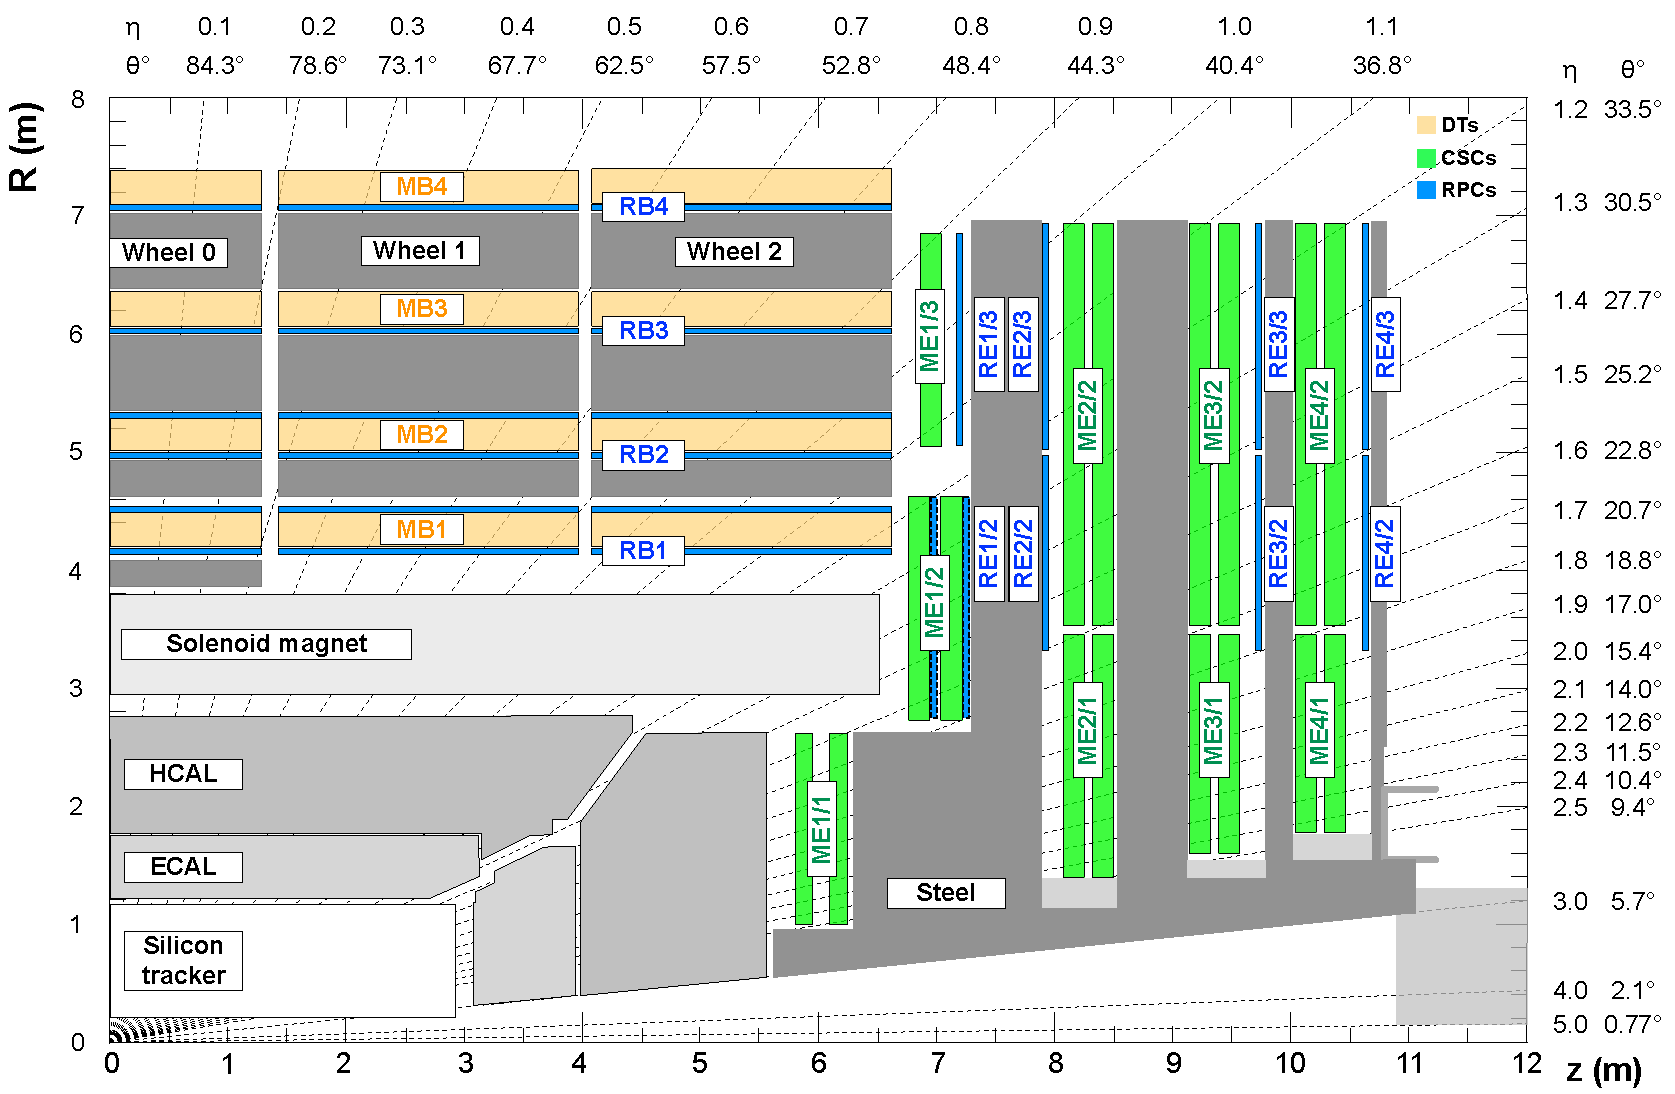
\includegraphics[width=0.85\textwidth]{fig/experiment/cms_crosssec.pdf}
  \caption{}
  \label{fig:CMSCrosssec}
\end{figure}

\subsection{Inner Tracking System}
\label{subsec:tracking}

\subsection{Calorimeters}
\label{subsec:calorimeter}

\subsection{Muon Tracking System}
\label{subsec:muonTrack}

\subsection{Trigger System and Data Acquisition}
\label{subsec:trigger}
